\documentclass{beamer}
%
% Choose how your presentation looks.
%
% For more themes, color themes and font themes, see:
% http://deic.uab.es/~iblanes/beamer_gallery/index_by_theme.html
%
\mode<presentation>
{
  \usetheme{NYU}      % or try Darmstadt, Madrid, Warsaw, ...
  \usecolortheme{default} % or try albatross, beaver, crane, ...
  \usefonttheme{default}  % or try serif, structurebold, ...
  \setbeamertemplate{navigation symbols}{}
  \setbeamertemplate{caption}[numbered]
} 

\usepackage[english]{babel}
\usepackage[utf8x]{inputenc}
\usepackage{multicol}
\usepackage{listings}
\usepackage{color}
\usepackage{booktabs}
\usepackage{tabularx}
\usepackage{cmap}
\usepackage[T1]{fontenc}

\definecolor{dkgreen}{rgb}{0,0.6,0}
\definecolor{gray}{rgb}{0.5,0.5,0.5}
\definecolor{mauve}{rgb}{0.58,0,0.82}

\lstset{frame=tb,
  language=Scala,
  aboveskip=3mm,
  belowskip=3mm,
  showstringspaces=false,
  columns=flexible,
  basicstyle={\small\ttfamily},
  numbers=none,
  numberstyle=\tiny\color{gray},
  keywordstyle=\color{blue},
  commentstyle=\color{dkgreen},
  stringstyle=\color{mauve},
  breaklines=true,
  breakatwhitespace=true,
  tabsize=3,
  mathescape=true
}



\title[BDAD Summer 2019 Symposium]{BDAD Summer 2019 Symposium}
%\author{Team: Cody Gilbert, Fang Han, Jeremy Lao}
\institute{NYU Courant, Computer Science}
\date{August 8, 2019}
\titlegraphic{\hfill
\includegraphics[height=1.5cm]{nyu_stacked_color}}

\begin{document}

\begin{frame}
  \titlepage
\end{frame}

% Uncomment these lines for an automatically generated outline.
%\begin{frame}{Outline}
%  \tableofcontents
%\end{frame}

\section{Big Data Applications Symposium}

\begin{frame}{Big Data Applications Symposium}

Project Name: Fair Lending Finder \vspace{3mm}

Team: 

\begin{itemize}
  \item Cody Gilbert
  \item Fang Han
  \item Jeremy Lao
\end{itemize}

Abstract:  \textit{We want to help people increase their chances of securing a mortgage related loan.  Our application will ask you for your details and provide you with the lender that is most likely to lend to you.  We trained our application using publicly available anonymized mortgage application information.}

\vskip 0.5cm

\end{frame}

\section{Fair Lending Finder}

\subsection{Motivation}

\begin{frame}{Motivation}

Who are the users of this application? 

\begin{itemize}
  \item General Public
  \item Banking Regulators 
\end{itemize}

Who will benefit from this application? 

\begin{itemize}
   \item Anyone that is looking for a mortgage loan
    \item Low to moderate income (LMI) borrowers
    \item People in states with high loan denial rates
\end{itemize}

Why is this application important? \vspace{2mm}

\begin{itemize}
  \item While there have been improvements in the mortgage lending process over the last decade, unconscious bias remains a factor in provisioning credit to average income borrowers.  Our application will help borrowers use that unconscious bias in their favor. 
\end{itemize}



\end{frame}

\begin{frame}{Goodness}

What steps were taken to assess the ''goodness`` of the analytic itself? \vspace{2mm}

We utilized publicly available Home Mortgage Disclosure Act (HMDA) data from 2007-2017 that contains over 207 million anonymized home mortgage application records to train a machine learning model on ''approved`` or ''denied`` mortgage applications.  \vspace{2mm}

We use the following features to train a Naive Bayes model:

    \begin{multicols}{3}
\begin{itemize}
  \item Loan Amount
  \item Applicant Income
  \item Race
  \item Gender
  \item Lender
  \item State
\end{itemize}
\end{multicols}

\end{frame}

\begin{frame}{Goodness (contd.)}

\begin{eqnarray*}
P(y=k) & = & \ \beta_0 loanAmt_{obs}  + \beta_1 applicantIncome_{obs} \\
& & + \delta_0 race + \delta_1 ethnicity  + \delta_2 gender  \\
& & + \delta_3 lender  +  \delta_4 state + \delta_5 year
\end{eqnarray*}

Where $\delta$ are dummy variables for the categorical variables and $\beta$ are coefficients. The outcome (k), approve or deny, $k \in 0,1$

\begin{table}[]
\begin{tabular}{|c|c|c|}
\hline
\textbf{MLModel}    & \textbf{Training/Test} & \textbf{AUC} \\ \hline
Logistic Regression & 80/20                  & 60\%         \\ \hline
SVM                 & 80/20                  & 59\%         \\ \hline
Naive Bayes         & 80/20                  & 79\%         \\ \hline
\end{tabular}
\caption{Model Evaluation}
\label{tab:my-table}
\end{table}



\end{frame}

\begin{frame}{Naive Bayes}

\begin{eqnarray*}
  P(y=k & | & loanAmt, applicantIncome \\
& & race, ethnicity, gender  \\
& & lender, state, year)
\end{eqnarray*}

\end{frame}


\begin{frame}{Actuation/Remediation}

What actuation or remediation actions are/could be performed by this application?  \vspace{3mm}

\begin{itemize}
  \item The loan applicant will use this application to determine the lender that will most likely extend credit, and the applicant can apply directly to that lender. 
  \item A banking regulator can use this to determine the lenders that are least likely to extend credit to LMI and minority communities 
\end{itemize}


\end{frame}

\begin{frame}{Data Sources}

\begin{table}[]
\begin{tabular}{|c|c|}
\hline
Name & HMDA Data Set         \\ \hline
Description                 & Anonymized mortgage loan application information          \\ \hline
Size of data        & $> 120$ GB              \\ \hline
\end{tabular}
\end{table}

\begin{table}[]
\begin{tabular}{|c|c|}
\hline
Name & Geospatial Data         \\ \hline
Description                 & Latitude and Longitude of States and Counties       \\ \hline
Size of data        & $> 100$ MB              \\ \hline
\end{tabular}
\end{table}


\begin{table}[]
\begin{tabular}{|c|c|}
\hline
Name & HMDA Panel Information         \\ \hline
Description                 & Lender metadata, such as parent ID and head office          \\ \hline
Size of data        & $> 100$ MB              \\ \hline
\end{tabular}
\end{table}

\end{frame}


\begin{frame}{Design Diagram}

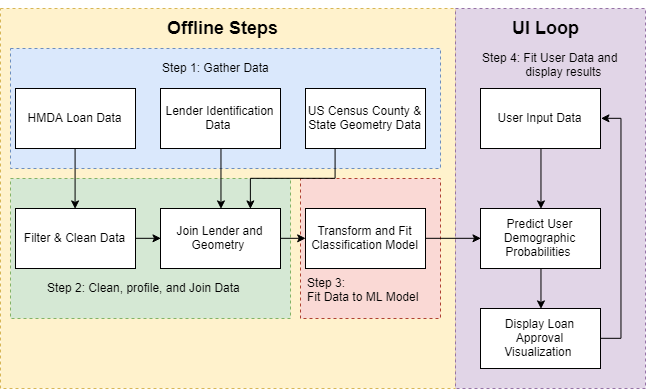
\includegraphics[width=\linewidth]{SparkDesignDiagram.png}

Platform(s) on which the application runs: \vspace{2mm}

NYU HPC Cluster (DUMBO)

\end{frame}

\begin{frame}[fragile]{Code Walkthrough}
\textbf{HMDA}


For data profiling, we originally ingested the data into a dataframe.  The entire profiling exercise would take 5-7 hours. 
\begin{lstlisting}

val dataForAnalysis = spark.read.format("csv").option("header", "true").  
                  option("inferSchema", "true").load(hdfsPath).
                  select("loan_amount_000s",...)
\end{lstlisting}

We changed our strategy and leveraged Spark Context RDDs to profile the data, reducing run-time to 1.5 hour: 

\begin{lstlisting}
   val dataForAnalysis = sc.textFile(hdfsPath)
   val reducedLoanAmtData = mapReduceFunc(dataForAnalysis, 7)
\end{lstlisting}

\end{frame}


\begin{frame}[fragile]{Code Walkthrough (contd.)}
\textbf{HMDA}

While dataframes have the .count() function, we had to write a custom function to perform count(): 

\begin{lstlisting}

def mapReduceFunc(dataForAnalysis : RDD[String], colNum : Integer) : RDD[String] = {
  val firstLine = dataForAnalysis.first() 
  val data = dataForAnalysis.filter(row => row != firstLine)
  val keyAmt = data.map(_.split(",")). map(c => (c(colNum),1)). reduceByKey((x,y) => x+y)
  val mrAmt = keyAmt.map(x => x._1.stripPrefix("\"").stripSuffix("\"") + "," + x._2)
  mrAmt
}
\end{lstlisting}

\end{frame}


\begin{frame}[fragile]{Code Walkthrough (contd.)}
\textbf{HMDA}

While dataframes preserve column names, you have to manually incorporate them in the RDD before saving as a .csv file:

\begin{lstlisting}

    val header: RDD[String]= sc.parallelize(List("loan_amount,frequency"))
     header.union(reducedLoanAmtData).saveAsTextFile(<path>)

\end{lstlisting}

\end{frame}



\begin{frame}[fragile]{Code Walkthrough (contd.)}
\textbf{HMDA - MLLib}

We developed the model using MLLib and saved the model to HDFS for our interactive application to use: 

\begin{lstlisting}

val indexer1 = new StringIndexer().
..
val encoder1 = new OneHotEncoder().
..
val assembler = new VectorAssembler().   //feature matrix
..
val pipeline = new Pipeline().setStages(Array(indexer,..,assembler,NaiveBayes))
...
val nbFinalModel  = cv.fit(hmdaInstitutionsBucketed)
nbFinalModel .save("<path>/HMDAModel")


\end{lstlisting}

\end{frame}

\begin{frame}[fragile]{Code Walkthrough (contd.)}
\textbf{HMDA - Visualization}

We had to use subplots in order to slice the data (gender, state, etc.)

\begin{lstlisting}

fig = make_subplots(
    rows=3, cols=2,
    column_widths=[0.5, 0.5], # corresponding to each row!
    row_heights=[0.25, 0.30, 0.45], # corresponding to each column!
    specs=[[{"type": "scatter", "rowspan": 2}, {"type": "scatter", "rowspan": 2}],[None ,None],
           [{"type": "scatter"}, {"type": "scatter"}]],
    subplot_titles=("Denial Rate Per Race", "Denial Rate Per Income Percentile", 
                    "Denial Rate Per Ethnicity", "Denial Rate Per Gender")
)

\end{lstlisting}

\end{frame}


\begin{frame}{Insights}

\begin{enumerate}

\item Loan Application amounts (sampled 2013 data) appear normally distributed between \$10,000 to \$500,000
\item Naive Bayes had the best AUC and the fastest performance time despite poor accuracy (79\% AUC)
\item Poor modeling results indicate that loans are not first-order dependent on applicant race, gender, or ethnicity

\end{enumerate}

\end{frame}



\begin{frame}{Obstacles}

\begin{enumerate}

\item Relatively large dataset, we needed to find ways to work around the speed of sparkSQL dataframes
\item The panel data was not as clean as we hoped - lenders are subsidiaries of bank holding companies (i.e. parent lender)
  \begin{itemize}
     \item Panel data information for some lenders was not uniformly entered from year to year
      \item Respondent IDs were not unique across regulating agencies (i.e. FDIC respondent 1 is not the same as Fed's respondent 1)
  \end{itemize}
\item Proper model iteration hindered by data size and relatively few available models

\end{enumerate}

\end{frame}



\begin{frame}{Summary}

This application will help you find the lender that will most likely extend credit based on your metadata.  It leverages historical information to learn lender patterns and bias.  

\end{frame}

\begin{frame}{Acknowledgements}

\begin{itemize}
  \item NYU HPC
  \item CFPB for making the data publicly available
  \item The Federal Reserve's and CFBP's data aggregators and collectors
  \item Professor McIntosh!

\end{itemize}

\end{frame}

\begin{frame}{References}

\footnotesize
\begin{itemize}
  \item S~Frumkin. \href{https://www.fdic.gov/regulations/examinations/supervisory/insights/siwin07/siwinter07-article4.pdf}{``HMDA Data: Identifying and Analyzing Outliers''}. \textit{Supervisory Insights, Winter 2007}.  Federal Deposit Insurance Corporation. 
 \item R. B. Avery, K. P. Brevoort, G. B. Canner. \href{https://ideas.repec.org/a/jre/issued/v29n42007p351-380.html
}{``Opportunities and Issues in Using HMDA Data''}. \textit{Journal of Real Estate Research, American Real Estate Society}. Vol. 29(4), pages 351-380. 2007.

\item \href{ https://catalog.data.gov/dataset/tiger-line-shapefile-2017-nation-u-s-current-county-and-equivalent-national-shapefile}{United States Census Bureau, Department of Commerce. TIGER/Line Shapefile, 2017, nation, U.S., Current County and Equivalent National Shapefile. Data.Gov. Updated June 2019. Retrieved July 2019.}

\item \href{https://catalog.data.gov/dataset/tiger-line-shapefile-2017-nation-u-s-current-state-and-equivalent-national  }{United States Census Bureau, Department of Commerce. TIGER/Line Shapefile, 2017, nation, U.S., Current State and Equivalent National. Data.Gov. Updated February 2019. Retrieved July 2019. }

\item Bissmark, Johan and Warnling, Oscar. \href{http://www.diva-portal.se/smash/get/diva2:1111045/FULLTEXT01.pdf}{The Sparse Data Problem Within Classification Algorithms: The Effect of Sparse Data on the Naïve Bayes Algorithm}. KTH, Datavetenskap, June 2017.

\item HMDA: \href{https://www.consumerfinance.gov/data-research/hmda/historic-data/}{Consumer Financial Protection Bureau public website of HMDA data}


\end{itemize}

\end{frame}

\begin{frame}{Demo!}
\textbf{DEMO}
\end{frame}

\begin{frame}{Thanks}

\textbf{Thank you!!}
\end{frame}
\end{document}
